\documentclass[a4paper]{article}

\usepackage{amsmath,amssymb}

\usepackage[english]{babel}
\usepackage[utf8x]{inputenc}

\usepackage{graphicx}
\usepackage[colorinlistoftodos]{todonotes}

\usepackage{theorem}

\usepackage{nameref, hyperref}

\usepackage{caption}
\usepackage{subcaption}


\usepackage[authoryear]{natbib}


\newenvironment{proof}{{\bf Proof:  }}{\hfill\rule{2mm}{2mm}}

\newtheorem{fact}{Fact}[section]
\newtheorem{lemma}[fact]{Lemma}
\newtheorem{theorem}[fact]{Theorem}
\newtheorem{definition}[fact]{Definition}
\newtheorem{corollary}[fact]{Corollary}
\newtheorem{proposition}[fact]{Proposition}
\newtheorem{claim}[fact]{Claim}
\newtheorem{exercise}[fact]{Exercise}

\newcommand{\RT}[1]{\marginpar{\footnotesize\color{red}RT: #1}}


%\usepackage[numbers]{natbib}
%\bibliographystyle{plainnat}
\usepackage{natbib}

\usepackage{tikz}
\usetikzlibrary{arrows}

\usepackage{algorithm}
\usepackage{algorithmic}
\usepackage{bm}

\DeclareMathOperator*{\argmin}{arg\,min}
\DeclareMathOperator*{\argmax}{arg\,max}

\renewcommand{\algorithmicrequire}{\textbf{Input:}}
\renewcommand{\algorithmicensure}{\textbf{Output:}}
\renewcommand{\hat}{\widehat}
\renewcommand{\tilde}{\widetilde}

% Defines a `datastore' shape for use in DFDs.  This inherits from a
% rectangle and only draws two horizontal lines.
\makeatletter
\pgfdeclareshape{datastore}{
  \inheritsavedanchors[from=rectangle]
  \inheritanchorborder[from=rectangle]
  \inheritanchor[from=rectangle]{center}
  \inheritanchor[from=rectangle]{base}
  \inheritanchor[from=rectangle]{north}
  \inheritanchor[from=rectangle]{north east}
  \inheritanchor[from=rectangle]{east}
  \inheritanchor[from=rectangle]{south east}
  \inheritanchor[from=rectangle]{south}
  \inheritanchor[from=rectangle]{south west}
  \inheritanchor[from=rectangle]{west}
  \inheritanchor[from=rectangle]{north west}
  \backgroundpath{
    %  store lower right in xa/ya and upper right in xb/yb
    \southwest \pgf@xa=\pgf@x \pgf@ya=\pgf@y
    \northeast \pgf@xb=\pgf@x \pgf@yb=\pgf@y
    \pgfpathmoveto{\pgfpoint{\pgf@xa}{\pgf@ya}}
    \pgfpathlineto{\pgfpoint{\pgf@xb}{\pgf@ya}}
    \pgfpathmoveto{\pgfpoint{\pgf@xa}{\pgf@yb}}
    \pgfpathlineto{\pgfpoint{\pgf@xb}{\pgf@yb}}
 }
}
\makeatother



\title{Robust LLG}

\date{\today}

\begin{document}
\maketitle

\section{Background and Overview}

Network analysis is becoming more and more widely used recently. In a general parametric framework, $G \sim f \in \mathcal{F} = \{f_{\theta} : \theta \in \Theta \}$, selecting a reasonable estimator $\hat{\theta}(G)$ for the unknown $\theta$ given a finite graph sample $\{G^{(1)}, \cdots, G^{(m)}\}$ is one of the most important tasks.

Consider the most basic setting, i.e. undirected and unweighted graphs with each edge independently distributed from a Bernoulli distribution, with the parameters to be the probabilities of the existence of edges between all pair of vertices.
Then the maximum likelihood estimate, which happens to be the entry-wise sample mean in this situation, is the uniformly minimum-variance unbiased estimator under the independent edge graph model (IEM) \citep{bollobas2007phase} without taking any graph structure into account. 
However, in a high dimensional situation, unbiased estimators often leads to inaccurate estimates with very high variance when the sample size is small. And for this basic setting we considered, the graphs are high dimensional object with $n^2$ parameters since $\Theta = [0, 1]^{n\times n}$, where $n$ denotes the number of vertices. Thus the MLE does not perform very well especially when there are only a few observations available, which is likely the case in real world.

Generally, by biasing towards low-rank structures carefully, the estimators will have a greatly reduced variances and win the bias-variance trade-off \citep{trunk1979problem}. Such improvement is not only important for the estimation itself, but also can help with other statistical inference procedures. For example, \citet{ginestet2014hypothesis} proposed a method to test if there is a difference between the networks of two groups of subjects. While hypothesis testing is the final goal, the estimation procedure is a key intermediate step and can be improved.

In order to improve the MLE considered above, the underlying graph structures are taken into account for exploiting the low-rank structure when constructing the estimator. One of the most important structures about the networks is the community structure in which vertices are clustered into different communities such that vertices within the same community behave similarly. The stochastic blockmodel (SBM) \citep{holland1983stochastic} captures such structural property strongly by assuming that vertices from the same block behave exactly the same.

As a generalization of the SBM, the latent position model (LPM) \citep{hoff2002latent} allows vertices to behave differently. Generally, the adjacencies between vertices depend on unobserved properties of the corresponding vertices. Thus under LPM, each vertex is associated with a latent position which influences the adjacencies for that vertex based on a link function. In this paper, we consider a special case of LPM, the random dot product graph (RDPG) \citep{young2007random, nickel2007random}, which has the dot product as the link function.

Recently, \citet{tang2016law} considers an estimator based on a low-rank approximation of the sample mean graph motivated by the RDPG model and proves that in the basic Bernoulli setting under SBM, the new estimator outperforms the element-wise sample mean since it decreases the overall asymptotic variance dramatically by smoothing towards the low-rank structure.

While \citet{tang2016law} demonstrate the advantage of the low-rank estimator for the unweighted graphs with Bernoulli distribution, the results are based on the assumption that graphs are observed without contaminations. However in practice there will be noise in the observed graphs. In this situation, there is no guarantee that the performance of the low-rank estimator is still better.

In this work, we are going to improve the estimation procedure in a contaminated scenario. Before we introduce the contaminations, it is helpful to extend the unweighted graphs with Bernoulli distribution to weighted graphs with a general distribution $f$. All the models we mentioned above (IEM, RDPG, and SBM) could be extended naturally and are discussed in details in Section~\ref{section:WIEM}, Section~\ref{section:WRDPG}, and Section~\ref{section:WSBM} respectively.

One of the most popular contamination model is the gross error model \citep{AIC:AIC690280519, bickel2001mathematical}. In a gross error model, we observe good measurement $G^* \sim f_P \in \mathcal{F}$ most of the time, while there are a few wild values $G^{**} \sim h_C \in \mathcal{H}$ when the gross errors occur.
As to the graphs, one way to generalize from the gross error model is to contaminate the entire graph with some small probability $\epsilon \in (0, 1)$, that is $G \sim (1-\epsilon) f_P + \epsilon h_C$. However, since all the models we consider are subsets of the IEM, it is more natural to consider the contaminations with respect to each edge, i.e. for $1 \le i, j \le n$, $G_{ij} \sim (1-\epsilon) f_{P_{ij}} + \epsilon h_{C_{ij}}$ with $f \in \mathcal{F}$ and $h \in \mathcal{H}$, where both $\mathcal{F}$ and $\mathcal{H}$ are one-parameter distribution families.

Under the contamination model, although we observe $G$ instead of $G^*$, estimating the parameters $P_{ij}$ ($1 \le i, j \le n$) of $f_{P_{ij}}$ in $\mathcal{F}$ is still our goal. We first prove that the low-rank estimator ($\widetilde{P}^{(1)}$ in Figure~\ref{fig:roadmap}) proposed in \citep{tang2016law} is still much better than the entry-wise MLE ($\hat{P}^{(1)}$ in Figure~\ref{fig:roadmap}) in terms of mean squared error when the observations are contaminated under proper conditions.

Furthermore, with contaminations, it is more preferable to use robust methods, like ML$q$E \citep{ferrari2010, qin2013maximum} considered in this paper. We prove that entry-wise ML$q$E ($\hat{P}^{(q)}$ in Figure~\ref{fig:roadmap}) improves the performance compared to entry-wise MLE ($\hat{P}^{(1)}$ in Figure~\ref{fig:roadmap}) whenever contamination is relatively large.

Similarly, in order to take advantage of the low-rank structure, we enforce a low-rank approximation on the entry-wise ML$q$E. We prove that, under proper assumptions, the new estimator ($\widetilde{P}^{(q)}$ in Figure~\ref{fig:roadmap}) not only inherits the robust property from ML$q$E ($\hat{P}^{(q)}$ in Figure~\ref{fig:roadmap}), but also wins the bias-variance trade-off by taking advantage of the low-rank structure.


\begin{figure}
\begin{center}
\hspace*{-0.2in}
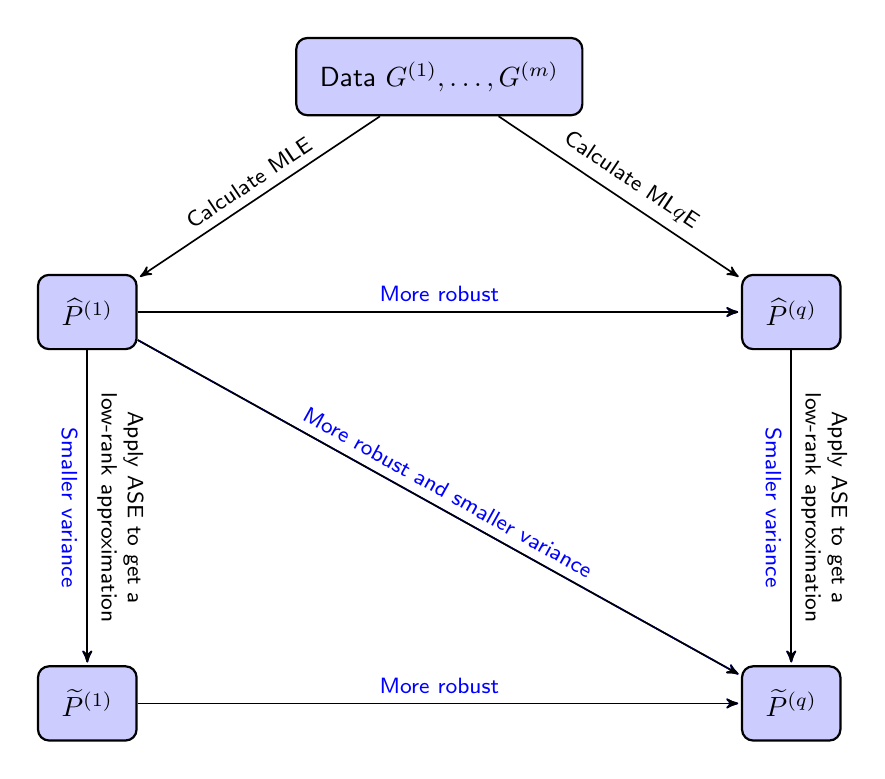
\begin{tikzpicture}[
  font=\sffamily,
  every matrix/.style={ampersand replacement=\&,column sep=2cm,row sep=2cm},
  block/.style={draw,thick,rounded corners,fill=blue!20,inner sep=.3cm},
  process/.style={draw,thick,circle,fill=blue!20},
  sink/.style={source,fill=green!20},
  datastore/.style={draw,very thick,shape=datastore,inner sep=.3cm},
  dots/.style={gray,scale=2},
  to/.style={->,>=stealth',shorten >=1pt,semithick,font=\sffamily\footnotesize},
  tofrom/.style={<->,>=stealth',shorten >=1pt,semithick,font=\sffamily\footnotesize},
  every node/.style={align=center}]

  % Position the nodes using a matrix layout
  \matrix{
  	\& \node[block] (Data) {Data $G^{(1)}, \dotsc, G^{(m)}$};\\
    \node[block] (MLE) {$\hat{P}^{(1)}$};
      \& \& \node[block] (MLqE) {$\hat{P}^{(q)}$};\\
	\\
    \node[block] (XMLE) {$\widetilde{P}^{(1)}$};
      \& \& \node[block] (XMLqE) {$\widetilde{P}^{(q)}$}; \\
  };

  % Draw the arrows between the nodes and label them.
  % \draw[to, blue] (Data) -- node[midway, sloped, below] {UMVUE w/o contamination} (MLE);
  \draw[to] (Data) -- node[midway, sloped, above] {Calculate MLE} (MLE);
  \draw[to] (Data) -- node[midway, sloped, above] {Calculate ML$q$E} (MLqE);
  \draw[to, blue] (MLE) -- node[midway,above] {More robust} (MLqE);
  \draw[to] (MLE) -- (MLqE);
  \draw[to, blue] (MLE) -- node[midway, sloped, below] {Smaller variance} (XMLE);
  \draw[to] (MLE) -- node[midway, sloped, above] {Apply ASE to get a \\ low-rank approximation} (XMLE);
  \draw[to, blue] (MLqE) -- node[midway, sloped, below] {Smaller variance} (XMLqE);
  \draw[to] (MLqE) -- node[midway, sloped, above] {Apply ASE to get a \\ low-rank approximation} (XMLqE);
  \draw[to, blue] (XMLE) -- node[midway,above] {More robust} (XMLqE);
  \draw[to] (XMLE) -- (XMLqE);
  \draw[to, blue] (MLE) -- node[midway, sloped, above] {More robust and smaller variance} (XMLqE);
  \draw[to] (MLE) -- (XMLqE);
\end{tikzpicture}
\end{center}
\caption{\label{fig:roadmap}Roadmap among the data and four estimators.}
\end{figure}


\section{Models}
\label{section:model}

For this work, we are in the scenario where $m$ weighted graphs on $n$ vertices are given in the adjacency matrices form $\{ A^{(t)} \} (t = 1, \dotsc, m)$. The graphs are undirected without self-loop, i.e. each $A^{(t)}$ is symmetric with zeros along the diagonal. Moreover, we assume the vertex correspondence is known across different graphs, so that vertex $i$ of the $t_1$-th graph corresponds to vertex $i$ of the $t_2$-th graph for any $i \in [n]$, $t_1, t_2 \in [m]$.

In this section, we present three nested models, the weighted independent edge model (WIEM) in Section~\ref{section:WIEM}, the weighted random dot product graph model (WRDPG) in Section~\ref{section:WRDPG}, and the weighted stochastic blockmodel (WSBM) as a WRDPG in Section~\ref{section:WSBM}. Moreover, we introduce a contaminated model based on Section~\ref{section:WSBM} in Section~\ref{section:Contamination}.

\subsection{Weighted Independent Edge Model}
\label{section:WIEM}

We first extend the definition of independent edge model (IEM) \citep{bollobas2007phase} to the weighted independent edge model (WIEM) with respect to a one-parameter family $\mathcal{F} = \{ f_{\theta} : \theta \in \Theta \subset \mathbb{R} \}$. Denote the graph parameters as a matrix $P \in \Theta^{n \times n} \subset \mathbb{R}^{n \times n}$. Then under a WIEM, each edge between vertex $i$ and vertex $j$ ($i < j$ because of symmetry) is distributed from $f_{P_{ij}}$ independently.

To see that an IEM is a special case of WIEM, just let $\mathcal{F}$ be the collection of Bernoulli distributions and let the graph parameters be a symmetric and hollow matrix $P \in [0, 1]^{n \times n}$.
Note that the graphs considered in this paper are undirected without self-loop, thus the parameter matrix $P$ needs to be symmetric and hollow. However, for convenience, we still define the parameters to be an $n$-by-$n$ matrix while only $n \choose 2$ of them are effective.


\subsection{Weighted Random Dot Product Graph}
\label{section:WRDPG}

The connectivity between two vertices in a graph generally depends on some hidden properties of the corresponding vertices. The latent position model proposed by \citet{hoff2002latent} captures such properties by assigning each vertex $i$ with a corresponding latent vector $X_i \in \mathbb{R}^d$. Conditioned on the latent vectors $X_i$ and $X_j$, the edge weight between vertex $i$ and vertex $j$ is independent of all other edges and depends only on $X_i$ and $X_j$ through a link function.

A special case of the latent position model is the random dot product graph model (RDPG) in which the link function is the inner product \citep{young2007random, nickel2007random}. Now we give a definition of the weighted random dot product graph (WRDPG) as a generalization of the weighted latent position model as following:
\begin{definition}[Weighted Random Dot Product Graph Model]
Consider a collection of one-parameter distributions $\mathcal{F} = \{ f_{\theta}, \theta \in \Theta \subset \mathbb{R} \}$. The weighted random dot product graph model (WRDPG) with respect to $\mathcal{F}$ is defined as following: Let $X \in \mathbb{R}^{n \times d}$ be such that $X = [X_1, X_2, \dotsc, X_n]^{\top}$, where $X_i \in \mathbb{R}^d$ for all $i \in [n]$. The matrix $X$ is random and satisfies $\mathbb{P}\left[ X_i^{\top} X_j \in \Theta \right] = 1$ for all $i, j \in [n]$. Conditioned on $X$, the entries of the adjacency matrix $A$ are independent and $A_{ij}$ is a random variable following distribution $f \in \mathcal{F}$ with parameter $ X_i^{\top} X_j $ for all $i \ne j \in [n]$.
\end{definition}
Under the WRDPG defined above, the parameter matrix $P = X X^T \in \mathbb{R}^{n \times n}$ is automatically symmetric because the link function is inner product. Moreover, to have symmetric graphs without self-loop, only $A_{ij}$ ($i < j$) are sampled while leaving the diagonals of $A$ to be all zeros.

%\begin{definition}
%Consider a collection of one-parameter distributions $\mathcal{F} = \{ F_{\theta}, \theta \in \Theta \subset \mathbb{R} \}$. Then the weighted random dot product graph model (WRDPG) with respect to $\mathcal{F}$ is defined as following: Let $\boldsymbol{X}, \boldsymbol{Y} \in \mathbb{R}^{n \times d}$ be such that $\boldsymbol{X} = [X_1, X_2, \cdots, X_n]^T$ and $\boldsymbol{Y} = [Y_1, Y_2, \cdots, Y_n]^T$, where $X_u, Y_u \in \mathbb{R}^d$ for all $u \in [n]$. The matrices $\boldsymbol{X}$ and $\boldsymbol{Y}$ are random and satisfy $\mathbb{P}\left[ \langle X_u, Y_v \rangle \in \Theta \right] = 1$ for all $u, v \in [n]$. Conditioned on $\boldsymbol{X}$ and $\boldsymbol{Y}$, the entries of the adjacency matrix $\boldsymbol{A}$ are independent and $\boldsymbol{A}_{uv}$ is a random variable with distribution $f \in \mathcal{F}$ with parameter $\langle X_u, Y_v \rangle$ for all $u \ne v \in [n]$.
%\end{definition}




\subsection{Weighted Stochastic Blockmodel as a Weighted Random Dot Product Graph}
\label{section:WSBM}

Community structure is an important property of graphs under which vertices are clustered into different communities such that vertices within the same community behave similarly. The stochastic blockmodel (SBM) proposed by \citet{holland1983stochastic} captures such property, where each vertex is assigned to one block and the connectivity between two vertices depends only on their respective block memberships.

Formally, the SBM is determined by the number of blocks $K$ (generally much smaller than the number of vertices $n$), block probability matrix $B \in [0, 1]^{K \times K}$, and the block assignment vector $\tau \in [K]^n$, where $\tau_i = k$ represents that vertex $i$ belongs to block $k$. Conditioned on the block membership $\tau$, the connectivity between vertex $i$ and vertex $j$ follows a Bernoulli distribution with parameter $B_{\tau_i, \tau_j}$. This can be easily generalized to the weighted stochastic blockmodel (WSBM), with the Bernoulli distributions replaced by a general distribution family one-parameter distributions $\mathcal{F} = \{ f_{\theta}, \theta \in \Theta \subset \mathbb{R} \}$ and the block probability matrix to be $B \in \Theta^{K \times K} \subset \mathbb{R}^{K \times K}$.

Since the RDPG/WRDPG setting motivates the low-rank estimator, all analysis in this work are based on such setting. In order to consider WSBM as a WRDPG, the block probability matrix $B$ needs to be positive semi-definite by the structure of WRDPG. From now on, we will denote the sub-model of WSBM with positive semi-definite $B$ as the WSBM.

Now consider the WSBM as a WRDPG with respect to $\mathcal{F} = \{ f_{\theta}, \theta \in \Theta \subset \mathbb{R} \}$. Let $d = 
\mathrm{rank}(B)$, then all vertices in block $k$ have shared latent position $\nu_k \in \mathbb{R}^{d}$, where $B = \nu \nu^{\top}$ and $\nu = [\nu_1, \dotsc, \nu_K]^{\top} \in \mathbb{R}^{K \times d}$. That is to say, $X_i = \nu_{\tau_i}$ and $A_{ij}$ $(i < j)$ is distributed from $f$ with parameter $B_{\tau_i, \tau_j} = \nu_{\tau_i}^{\top} \nu_{\tau_j}$. Here the parameter matrix $P \in \mathbb{R}^{n \times n}$ is symmetric, hollow, and satisfies $P_{ij} = X_i^{\top} X_j = \nu_{\tau_i}^{\top} \nu_{\tau_j} = B_{\tau_i, \tau_j}$.

In order to generate $m$ graphs under this model with known vertex correspondence, we first sample $\tau$ from the categorical distribution with parameter $\rho = [\rho_1, \cdots, \rho_K]^{\top}$ with $\rho_k \in (0, 1)$ and $\sum_{k = 1}^{K} \rho_k = 1$, and keep $\rho$ fixed when sampling all $m$ graphs. Then $m$ symmetric and hollow graphs are sampled such that conditioning on $\tau$, the adjacency matrices are distributed entry-wise independently as $A^{(t)}_{ij} \stackrel{ind}{\sim} f_{B_{\tau_i, \tau_j}} = f_{P_{ij}}$ for each $1 \le t \le m$, $1 \le i < j \le n$.


\begin{itemize}
\item Here is an example of the WSBM. (Figure for simulation)
\end{itemize}

\subsection{Weighted Stochastic Blockmodel as a Weighted Random Dot Product Graph with Contaminations}
\label{section:Contamination}

In practice, we can hardly get data accurately. So there will always be noise in the observations, which deviates from our general model assumptions. In order to incorporate this effect, a contamination model, the gross error model \citep{AIC:AIC690280519, bickel2001mathematical}, is considered in this work.

Generally in a gross error model, we observe good measurement $G^* \sim f_P \in \mathcal{F}$ most of the time, while there are a few wild values $G^{**} \sim h_C \in \mathcal{H}$ when the gross errors occur. Here $P$ and $C$ represent the respective parameter matrices of the two distribution families.
As to the graphs, one way to generalize from the gross error model is to contaminate the entire graph with some small probability $\epsilon \in (0, 1)$, that is $G \sim (1-\epsilon) f_P + \epsilon h_C$. However, since all the models we consider are subsets of the WIEM, it is more natural to consider the contaminations with respect to each edge, i.e. for $1 \le i <  j \le n$, $G_{ij} \sim (1-\epsilon) f_{P_{ij}} + \epsilon h_{C_{ij}}$ with $f \in \mathcal{F}$ and $h \in \mathcal{H}$, where both $\mathcal{F}$ and $\mathcal{H}$ are one-parameter distribution families.

In this paper, we assume that when gross errors occur, the connectivity also follows the WSBM as a WRDPG. That is, the contamination distributions $h_{C_{ij}}$ are also from the same one-parameter family $\mathcal{F}$ as well as $f_{P_{ij}}$. For clarity, we will introduce the sampling procedure when the contamination has the same block structure. However, the parameter matrix $C$ for the contamination does not need to have the same block structure as $P$ in general.

To generate $m$ graphs under this contamination model with known vertex correspondence, we first sample $\tau$ from the categorical distribution with parameter $\rho$ and keep it fixed for all $m$ graphs as in Section \ref{section:WSBM}. Then $m$ symmetric and hollow graphs $G^{(1)}, \dotsc, G^{(m)}$ are sampled such that conditioning on $\tau$, the adjacency matrices are distributed entry-wise independently as $A^{(t)}_{ij} \stackrel{ind}{\sim} (1-\epsilon) f_{P_{ij}} + \epsilon f_{C_{ij}}$ for each $1 \le t \le m$, $1 \le i < j \le n$. Here $\epsilon$ is the probability of an edge to be contaminated, $P$ is the parameter matrix as in Section \ref{section:WSBM}, and $C$ is the parameter matrix for contaminations.



\section{Estimators}

Under any model introduced in Section~\ref{section:model}, our goal is to estimate the parameter matrix $P$ based on the $m$ observations $A^{(1)}, \dotsc, A^{(m)}$. Especially when under the contamination model, although there are other parameters like $\epsilon$ and $C$, our goal is still to estimate the uncontaminated parameter matrix $P$. In this section, we present four estimators as in Figure~\ref{fig:roadmap}, i.e. the standard entry-wise MLE $\hat{P}^{(1)}$, the low-rank approximation of the entry-wise MLE $\widetilde{P}^{(1)}$, the entry-wise robust estimator ML$q$E $\hat{P}^{(q)}$, and the low-rank approximation of the entry-wise ML$q$E $\widetilde{P}^{(q)}$. Since the observed graphs are symmetric and hollow with a symmetric parameter matrix of the model, we do not care about the estimate of the diagonal of $P$. However, the estimate itself should be at least symmetric.

\subsection{Entry-wise Maximum Likelihood Estimator $\hat{P}^{(1)}$}

Under the WIEM, the most natural estimator is the MLE, which happens to be the element-wise MLE $\hat{P}^{(1)}$ in this case.
Moreover, when $\mathcal{F}$ is a one-parameter exponential family, for instance Bernoulli and Exponential, the entry-wise MLE $\hat{P}^{(1)}$ is uniformly minimum-variance unbiased estimator, i.e. it has the smallest variance among all unbiased estimators. In addition, it satisfies many good asymptotic properties as the number of graphs $m$ goes to infinity.
However, in high dimensional situations like this, the entry-wise MLE often leads to inaccurate estimates with very high variance when the sample size $m$ is small. Also, it does not exploit any graph structure. The performance will not get any better when the number of vertices in each graph $n$ increases since it is an entry-wise estimator. Moreover, if the graphs are actually distributed under a WRDPG or a WSBM, then the entry-wise MLE is no longer the MLE any more and the performance can be very poor.


\subsection{Estimator $\widetilde{P}^{(1)}$ Based on Adjacency Spectral Embedding of $\hat{P}^{(1)}$}

Motivated by the low-rank structure of the parameter matrix $P$ in WRDPG, we consider the estimator $\widetilde{P}^{(1)}$ proposed by \citet{tang2016law} based on the spectral decomposition of $\hat{P}^{(1)}$. The estimator $\widetilde{P}^{(1)}$ is similar to the estimator proposed by \citet{chatterjee2015matrix} with adjustment for the specific estimation task, including a different dimension selection technique discussed in Section~\ref{section:dim_select} and a diagonal augmentation procedure discussed in Section~\ref{section:diag_aug}. The construction procedure of $\widetilde{P}^{(1)}$ consists of several steps, which will be introduced respectively in the following subsections.

\subsubsection{Rank-$d$ Approximation}

Given a dimension $d$, we consider $\widetilde{P}^{(1)} = \mathrm{lowrank}_d(\hat{P}^{(1)})$ as the best rank-$d$ positive semi-definite approximation of $\hat{P}^{(1)}$. To find such best approximation, first calculate the eigen-decomposition of the symmetric matrix $\hat{P}^{(1)} = \hat{U} \hat{S} \hat{U}^{\top} + \widetilde{U} \widetilde{S} \widetilde{U}^{\top}$, where $\hat{S}$ is the diagonal matrix with the largest $d$ eigenvalues of $\hat{P}^{(1)}$, and $\hat{U}$ has the corresponding eigenvectors as each column. Similarly, $\tilde{S}$ is the diagonal matrix with non-increasing entries along the diagonal corresponding to the rest $n - d$ eigenvalues of $\hat{P}^{(1)}$, and $\tilde{U}$ has the columns given by the corresponding eigenvectors.
The $d$-dimensional adjacency spectral embedding (ASE) of $\hat{P}^{(1)}$ is given by $\hat{X}=\hat{U} \hat{S}^{1/2}\in \mathbb{R}^{n \times d}$.
Based on the ASE result, we have the best rank-$d$ positive semi-definite approximation of $\hat{P}^{(1)}$ to be $\widetilde{P}^{(1)} = \hat{X} \hat{X}^{\top}=\hat{U}\hat{S}\hat{U}^{\top}$.
In the RDPG setting, \citet{sussman2014consistent} proved that each row of $\hat{X}$ can accurately estimate the the latent position for each vertex up to an orthogonal transformation. We will analyze its performance under the WRDPG setting in Section \ref{section:theory}.

Here, we restate the algorithm in \citep{tang2016law} to give the detailed steps of computing this low-rank approximation of a general $n$-by-$n$ symmetric matrix $A$ in Algorithm~\ref{algo:lowrank}.
\begin{algorithm}[H]
\caption{Algorithm to compute the rank-$d$ approximation of a matrix.}
\label{algo:lowrank}
\begin{algorithmic}[1]
\REQUIRE Symmetric matrix $A\in \mathbb{R}^{n \times n}$ and dimension $d\leq n$.
\ENSURE $\mathrm{lowrank}_d(A)\in \mathbb{R}^{n \times n}$
\STATE Compute the algebraically largest $d$ eigenvalues of $A$, $s_1\geq s_2\ge \dotsc \ge s_d$ and corresponding unit-norm eigenvectors $u_1,u_2,\dotsc,u_d\in \mathbb{R}^n$;
\STATE Set $\hat{S}$ to the $d\times d$ diagonal matrix $\mathrm{diag}(s_1,\dotsc,s_d)$;
\STATE Set $\hat{U} = [u_1,\dotsc,u_d]\in \mathbb{R}^{n \times d}$;
\STATE Set $\mathrm{lowrank}_d(A)$ to $\hat{U}\hat{S}\hat{U}^{\top}$;
\end{algorithmic}
\end{algorithm}


\subsubsection{Dimension Selection}
\label{section:dim_select}

Although Algorithm~\ref{algo:lowrank} gives us a way to calculate the best rank-$d$ positive semi-definite approximation of a general symmetric matrix $A$, it does not tell us how to select a proper dimension $d$. If we choose a relatively small dimension $d$, the estimator based on approximation will fail to catch much important information. On the other hand, when $d$ is too large, the approximation will contain too much noise and also lead to a bad estimate. So a carefully selected dimension $d$ is a key part of a good estimation.

A general idea of selecting the dimension $d$ is to analyze the ordered eigenvalues and looking for the ``gap'' or ``elbow'' in the scree-plot.
In 2006, \citet{zhu2006automatic} proposed an automatic method for finding the gap in the scree-plot by only looking at the eigenvalues based on a Gaussian mixture model. This method provides multiple choices based on different elbow. In this paper, to avoid under-estimating the dimension, which is often much more harmful than over-estimating it, we always choose the 3rd elbow.

Although it is always challenge to select a proper dimension, based on the results of real data experiment in Section~\ref{section:real_data}, a wide range of dimensions will lead to a fairly good results. Thus a proper dimension selection method can be applied directly without carefully tuning the parameter, which makes the estimator much more useful in practice.



\subsubsection{Diagonal Augmentation}
\label{section:diag_aug}

Since the graphs considered in this paper have no self-loops, all the adjacency matrices $A^{(t)}$ ($1 \le t \le m$) are hollow, i.e. all diagonal entries are zeros. Thus the diagonal of the parameter matrix $P$ does not matter since all off-diagonal entries are independent of them conditioned on the off-diagonal entries of $P$.

However, unlike the entry-wise estimators, e.g. $\hat{P}^{(1)}$, the ones which take advantage of the graph structure need the information from the diagonals. As a result, the zero diagonals of the observed graphs will lead to unnecessary biases in those estimates.

To compensate for such unnecessary biases, \citet{marchette2011vertex} suggested to use the average of the non-diagonal entries of the corresponding row as the diagonal entry before embedding. Also, \citet{scheinerman2010modeling} proposed an iterative method, which gives a different approach to resolve such issue.

As suggested in \citep{tang2016law}, in this work we are going to combine both ideas by first using Marchette's row-averaging method (see Step 3 of Algorithm~\ref{algo:basic}) and then another one-step Scheinerman's iterative method (see Step 6 of Algorithm~\ref{algo:basic}).


\begin{algorithm}[H]
\caption{Algorithm to compute $\widetilde{P}^{(1)}$}
\label{algo:basic}
\begin{algorithmic}[1]
\REQUIRE Symmetric adjacency matrices $A^{(1)}, A^{(2)}, \dotsc, A^{(m)}$, with each $A^{(t)} \in \mathbb{R}^{n \times n}$
\ENSURE Estimate $\widetilde{P}^{(1)} \in \mathbb{R}^{n \times n}$
\STATE Calculate the entry-wise MLE $\hat{P}^{(1)}$;
\STATE Calculate the scaled degree matrix $D = \mathrm{diag}(\hat{P}^{(1)} \bm{1})/(n-1)$;
\STATE Select the dimension $d$ based on the eigenvalues of $\hat{P}^{(1)} + D$; (see Section~\ref{section:dim_select})
\STATE Set $Q$ to $\mathrm{lowrank}_d(\hat{P}^{(1)} + D)$; (see Algorithm~\ref{algo:lowrank})
\STATE Set $D^{\prime}$ to $ \mathrm{diag}(Q)$, the diagonal matrix with diagonal matching $Q$; 
\STATE Set $Q^{\prime}$ to $\mathrm{lowrank}_d(Q + D^{\prime})$; (see Algorithm~\ref{algo:lowrank})
\STATE Set $\widetilde{P}^{(1)}$ with each entry $\widetilde{P}^{(1)}_{ij} = \min( \hat{P}^{(1)}_{ij}, \max(Q^{\prime}_{ij}, 0))$.
\end{algorithmic}
\end{algorithm}

\begin{itemize}
\item Truncation procedure. Need reasonable explanation here.
\end{itemize}

By combining the key parts introduced above, we give the detailed description for calculating the estimator $\widetilde{P}^{(1)}$ with dimension selection method and diagonal augmentation procedure in Algorithm~\ref{algo:basic}.




\subsection{Entry-wise Maximum L$q$-likelihood Estimator $\hat{P}^{(q)}$}

The MLE is asymptotically efficient, i.e. when sample size is large enough, the MLE is at least as accurate as any other estimator. However, when the sample size is moderate, robust estimators always outperforms MLE in terms of mean squared error by winning the bias-variance tradeoff. Moreover, under contamination models, robust estimators can even beat MLE asymptotically since they are designed to be not unduly affected by the outliers. And now we are going to consider one robust estimator, i.e. the maximum L$q$-likelihood estimator (ML$q$E) proposed by \citet{ferrari2010}.

Let $X_1, \dotsc, X_m$ be sampled from $f_{\theta_0} \in \mathcal{F} = \{ f_{\theta}, \theta \in \Theta \}$, $\theta_0 \in \Theta$. Then the maximum L$q$-likelihood estimate ($q > 0$) of $\theta_0$ based on the parametric model $\mathcal{F}$ is defined as
\[
	\hat{\theta}_{\mathrm{ML}q\mathrm{E}} = \argmax_{\theta \in \Theta} \sum_{i=1}^m L_q[f_{\theta}(X_i)],
\]
where $L_q(u) = (u^{1-q} - 1)/(1- q)$.
Note that $L_q(u) \to \log(u)$ when $q \to 1$. Thus ML$q$E is a generalization of MLE.
Moreover, define
\[
	U_{\theta}(x) = \nabla_{\theta} \log f_{\theta}(x)
\]
and
\[
	U^{\star}_{\theta}(x; q) = U_{\theta}(x) f_{\theta}(x)^{1-q}.
\]
Then the ML$q$E $\hat{\theta}_{\mathrm{ML}q\mathrm{E}}$ can also be seen as a solution to the equation
\[
	\sum_{i=1}^m U^{\star}_{\theta}(X_i; q) = 0.
\]
This form interprets $\hat{\theta}_{\mathrm{ML}q\mathrm{E}}$ as a solution to the weighted likelihood equation. The weights $f_{\theta}(x)^{1-q}$ are proportional to the $(1-q)$th power of the corresponding probability. Specifically, when $0 < q < 1$, the ML$q$E puts less weight on the data points which do not fit the current distribution well. Equal weights happens when $q=1$ and lead to the MLE.

Under the WIEM, we can calculate the robust entry-wise ML$q$E $\hat{P}^{(q)}$ based on the adjacency matrices $A^{(1)}, \dotsc, A^{(m)}$. Note that $\hat{P}^{(1)}$, the entry-wise MLE, is a special case of entry-wise ML$q$E $\hat{P}^{(q)}$ when $q = 1$. That is what the superscriptions $q$ and $1$ mean.



\subsection{Estimator $\widetilde{P}^{(q)}$ Based on Adjacency Spectral Embedding $\hat{P}^{(q)}$}

Intuitively, the low-rank structure of the parameter matrix $P$ in WRDPG should be preserved more or less in the entry-wise ML$q$E $\hat{P}^{(q)}$. Thus, in order to take advantage of such low-rank structure as well as the robustness, we apply the similar idea here as in building $\widetilde{P}^{(1)}$, i.e. enforce a low-rank approximation on the entry-wise ML$q$E matrix $\hat{P}^{(q)}$ to get $\widetilde{P}^{(q)}$. As in Algorithm~\ref{algo:basic}, we apply the same dimension selection method and diagonal augmentation procedure. The only change is to substitute $\hat{P}^{(1)}$ by $\hat{P}^{(q)}$. The details of the algorithm is shown in Algorithm~\ref{algo:basic_q}.

\begin{algorithm}[H]
\caption{Algorithm to compute $\widetilde{P}^{(q)}$}
\label{algo:basic_q}
\begin{algorithmic}[1]
\REQUIRE Symmetric adjacency matrices $A^{(1)}, A^{(2)}, \dotsc, A^{(m)}$, with each $A^{(t)} \in \mathbb{R}^{n \times n}$
\ENSURE Estimate $\widetilde{P}^{(q)} \in \mathbb{R}^{n \times n}$
\STATE Calculate the entry-wise ML$q$E $\hat{P}^{(q)}$;
\STATE Calculate the scaled degree matrix $D = \mathrm{diag}(\hat{P}^{(q)} \bm{1})/(n-1)$;
\STATE Select the dimension $d$ based on the eigenvalues of $\hat{P}^{(q)} + D$; (see Section~\ref{section:dim_select})
\STATE Set $Q$ to $\mathrm{lowrank}_d(\hat{P}^{(q)} + D)$; (see Algorithm~\ref{algo:lowrank})
\STATE Set $D^{\prime}$ to $ \mathrm{diag}(Q)$, the diagonal matrix with diagonal matching $Q$; 
\STATE Set $Q^{\prime}$ to $\mathrm{lowrank}_d(Q + D^{\prime})$; (see Algorithm~\ref{algo:lowrank})
\STATE Set $\widetilde{P}^{(q)}$ with each entry $\widetilde{P}^{(q)}_{ij} = \min( \hat{P}^{(q)}_{ij}, \max(Q^{\prime}_{ij}, 0))$.
\end{algorithmic}
\end{algorithm}

%\begin{figure}
%\centering
%\begin{subfigure}{.5\textwidth}
%  \centering
%  \includegraphics[width=1.2\linewidth]{SBM_P.png}
%\end{subfigure}%
%\begin{subfigure}{.5\textwidth}
%  \centering
%  \includegraphics[width=1.2\linewidth]{SBM_A.png}
%\end{subfigure}
%\caption{Example illustrating the SBM. The figure on the left is the probability matrix $P$ that follows a SBM with $K = 5$ blocks; The other figure shows the adjacency matrix $A$ for 200 vertices generated from the SBM with probability matrix $P$.}
%\label{fig:SBM_example}
%\end{figure}

\section{Theoretical Results}
\label{section:theory}
In this section, for illustrative purpose, we are going to present theoretical results when the contamination model introduced in Section~\ref{section:Contamination} is based on exponential distributions. That is $\mathcal{F} = \{ f_{\theta}(x) = \frac{1}{\theta} e^{-x/\theta}, \theta \in [0, R] \subset \mathbb{R} \}$, where $R > 0$ is a constant. The results can be extended to a general situation with proper assumptions, which will be discussed in Section~\ref{section:extension}.

For clarity, we restate the model settings discussed in Section~\ref{section:Contamination}. Consider the SBM with parameter $B$ and $\rho$. First sample the block membership $\tau$ from the categorical distribution with parameter $\rho$ and keep it fixed for all $m$ graphs. Conditioned on this $\tau$ we sampled, the probability matrix $P$ then satisfies $P_{ij} = B_{\tau_i, \tau_j}$. In this section, we assume the contamination has the same block membership $\tau$, thus the contamination matrix $C \in \mathbb{R}^{n \times n}$ has the same block structure as $P$. Note that this is not necessary for the result. Different block structure can lead to the same result since the rank is still finite. Denote $\epsilon$ as the probability of an edge to be contaminated. Then $m$ symmetric graphs $G^{(1)}, \dotsc, G^{(m)}$  are sampled such that conditioning on $\tau$, the adjacency matrices are distributed entry-wise independently as $A^{(t)}_{ij} \stackrel{ind}{\sim} (1-\epsilon) f_{P_{ij}} + \epsilon f_{C_{ij}}$ for each $1 \le t \le m$, $1 \le i < j \le n$. 

Under such setting, we analyze the performance of all four estimators based on $m$ adjacency matrices for estimating the probability matrix $P$ in terms of the mean squared error. When comparing two estimators, we mainly focus on both asymptotic bias and asymptotic variance. Note that all the results in this section are entry-wise, which can easily lead to a result of the total MSE for the entire matrix.

We only present the most important results in this section. The proofs with more results are in the Appendix.

\subsection{$\hat{P}^{(1)}$ vs. $\hat{P}^{(q)}$}
\label{section:MLEvsMLqE}
We first compare the performance between the entry-wise MLE $\hat{P}^{(1)}$ and the entry-wise ML$q$E $\hat{P}^{(q)}$. Without using the graphs structure, the asymptotic results for these two estimators are in terms of the number of graphs $m$, not the number of vertices $n$ within each graph.

\begin{lemma}
\label{lemma:ELqlEMLE}
For any $0 < q < 1$, there exists $C_0(P_{ij}, \epsilon, q) > 0$ such that under the contaminated model with $C > C_0(P_{ij}, \epsilon, q)$,
\[
	\lim_{m \to \infty} \left| E[\hat{P}^{(q)}_{ij}] - P_{ij} \right| < 
    \lim_{m \to \infty} \left| E[\hat{P}^{(1)}_{ij}] - P_{ij} \right|,
\]
for $1 \le i, j \le n$ and $i \ne j$.
\end{lemma}

Lemma~\ref{lemma:ELqlEMLE} shows that the entry-wise ML$q$E $\hat{P}^{(q)}$ has smaller bias for estimating $P$ asymptotically compared to the entry-wise MLE $\hat{P}^{(1)}$ under proper conditions. Although we put restrictions on the parameter matrix $C$ in the assumption, to have the current result about asymptotic bias, we only need to satisfy the inequality $\epsilon (C_{ij} - P_{ij}) > (1 - q) P_{ij}$. This condition actually requires the contamination of the model is large enough (either large contamination parameter matrix, or more likely to encounter an outlier). From a different perspective, it also requires $\hat{P}^{(q)}$ to be robust enough with respect to the contamination. Thus besides the current condition for $C$, equivalently, we can also replace it by the assumption of a large enough $\epsilon$ or a small enough $q$.

\begin{lemma}
\label{lemma:VarLqlVarMLE}
\[
	\lim_{m \to \infty} \mathrm{Var}(\hat{P}^{(1)}_{ij})
    = \lim_{m \to \infty} \mathrm{Var}(\hat{P}^{(q)}_{ij}) = 0,
\]
for $1 \le i, j \le n$.
\end{lemma}

By this lemma, both estimators have asymptotic variances equal zero as the number of graphs $m \to \infty$. Under the mixture model, the result for MLE follows the central limit theorem immediately, while the ML$q$E result is not trivial. Our proof is based on the minimum contrast estimates (more details later).

As a result, $\hat{P}^{(q)}$ reduces the bias while keeping variance the same asymptotically compared to $\hat{P}^{(1)}$. Thus in terms of MSE, $\hat{P}^{(q)}$ is a better estimator than $\hat{P}^{(1)}$ when the number of graphs $m$ is large with enough contaminations.

\subsection{$\hat{P}^{(1)}$ vs. $\widetilde{P}^{(1)}$}
Then we are going to analyze the effect of the ASE procedure applied to the entry-wise MLE $\hat{P}^{(1)}$ under the contamination model.

\begin{corollary}
\label{cor:L1Consistent}
Assuming that $m = O(n^b)$ for any $b > 0$, then the estimator based on ASE of MLE has the same entry-wise asymptotic bias as MLE, i.e.
\[
	\lim_{n \to \infty} \mathrm{Bias}(\widetilde{P}_{ij}^{(1)}) = \lim_{n \to \infty} E[\widetilde{P}_{ij}^{(1)}] - P_{ij} = \lim_{n \to \infty} E[\hat{P}^{(1)}_{ij}] - P_{ij}
    = \lim_{n \to \infty} \mathrm{Bias}(\hat{P}_{ij}^{(1)}).
\]
\end{corollary}

To prove the the corollary, we first give a bound on the $2$-norm of $\hat{P}^{(1)} - E[\hat{P}^{(1)}]$ by the matrix Bernstein inequality \cite{tropp2012user}. Since we are under the RDPG setting, $E[\hat{P}^{(1)}]$ still has finite rank, which makes the embedding reasonable. Then we approximate $U^T \hat{U}$ by an orthogonal matrix $W^{\star}$ based on Davis-Kahan theorem \cite{davis1970rotation}, where $U$ and $\hat{U}$ are the eigen-spaces for $E[\hat{P}^{(1)}]$ and $\hat{P}^{(1)}$ respectively. Then we can analyze the bounds much more easily by interchanging $U^T \hat{U}$ in the matrix multiplications. As a result, we can get the bound between the estimates of the latent positions and the true latent positions up to an orthogonal transformation in terms of $2 \to \infty$ norm. Corollary \ref{cor:L1Consistent} then follows by selecting the parameter carefully in the analysis.

Corollary \ref{cor:L1Consistent} says that when $m = O(n^b)$ for any $b > 0$, the ASE procedure applied to $\hat{P}^{(1)}$ will not affect the asymptotic bias for estimating $P$.
In this case, the asymptotic relative efficiency (ARE) \cite{serfling2011asymptotic} provides a good way to compare these two estimators. The definition proposed by Serfling in 2009 is based on unbiased estimators, here we extend it a little bit such that it can be measure two estimators which have the same asymptotic bias.
\begin{definition}
For any parameter $\theta$ of a distribution $f$, and for estimators $\hat{\theta}^{(1)}$ and $\hat{\theta}^{(2)}$ approximately $N(\theta^{\prime}, V_1(f)/n)$ and $N(\theta^{\prime}, V_2(f)/n)$ respectively, the ARE of $\hat{\theta}^{(2)}$ to $\hat{\theta}^{(1)}$ is given by
\[
	\mathrm{ARE}(\hat{\theta}^{(2)}, \hat{\theta}^{(1)}) = \frac{V_1(f)}{V_2(f)}.
\]
\end{definition}

In our situation, we can compare the performance between $\widetilde{P}^{(1)}$ and $\hat{P}^{(1)}$ entry-wise based on the ARE, which can be written as $\mathrm{ARE}(\widetilde{P}^{(1)}, \hat{P}^{(1)}) = \lim_{n \to \infty} \mathrm{Var}(\widetilde{P}_{ij}^{(1)})/\mathrm{Var}(\hat{P}_{ij}^{(1)})$. First, we analyze the order of $\mathrm{Var}(\widetilde{P}_{ij}^{(1)})$ in the following theorem.
\begin{theorem}
\label{thm:VarASEL1}
Assuming that $m = O(n^b)$ for any $b > 0$, then $\mathrm{Var}((\hat{Z}_i^T \hat{Z}_j)_{\mathrm{tr}}) = O(m^{-1} n^{-1} (\log n)^3)$.
\end{theorem}

The tools we use to prove this theorem is the same as for Corollary \ref{cor:L1Consistent}. Combined with Lemma \ref{lemma:VarLqlVarMLE}, we directly have the ARE results as following:
\begin{theorem}
\label{thm:AREL1}
For fixed $m$, $1 \le i, j \le n$ and $i \ne j$,
\[
	\frac{\mathrm{Var}(\widetilde{P}_{ij}^{(1)})}{\mathrm{Var}(\hat{P}_{ij}^{(1)})}
    = O(n^{-1} (\log n)^3).
\]
Thus
\[
	\mathrm{ARE}(\hat{P}_{ij}^{(1)}, \widetilde{P}_{ij}^{(1)}) = 0.
\]
Furthermore, as long as $m$ goes to infinity of order $O(n^b)$ for any $b > 0$,
\[
	\mathrm{ARE}(\hat{P}_{ij}^{(1)}, \widetilde{P}_{ij}^{(1)}) = 0.
\]
\end{theorem}

Theorem \ref{thm:AREL1} tells us that whenever $m = O(n^b)$ for any $b > 0$, i.e. $m$ is fixed or it grows not faster than polynomial with respect to $n$, the order of the ARE is $O(n^{-1} (\log n)^3)$, which converges to 0 when $n \to \infty$. An interesting fact here is that this bound of the ARE does not depend on $m$.

As a result, the ASE procedure applied to the entry-wise MLE $\hat{P}^{(1)}$ helps reduce the variance while keeping the bias asymptotically, leading to a better estimate $\widetilde{P}^{(1)}$ for $P$ in terms of MSE.



\subsection{$\hat{P}^{(q)}$ vs. $\widetilde{P}^{(q)}$}

Similarly, we now analyze the effect of the ASE procedure applied to the entry-wise ML$q$E $\hat{P}^{(q)}$ under the contamination model.

\begin{corollary}
\label{cor:LqConsistent}
Assuming that $m = O(n^b)$ for any $b > 0$, then the estimator based on ASE of ML$q$E has the same entry-wise asymptotic bias as ML$q$E, i.e.
\[
	\lim_{n \to \infty} \mathrm{Bias}(\widetilde{P}_{ij}^{(q)}) = \lim_{n \to \infty} E[\widetilde{P}_{ij}^{(q)}] - P_{ij} = \lim_{n \to \infty} E[\hat{P}^{(q)}_{ij}] - P_{ij}
    = \lim_{n \to \infty} \mathrm{Bias}(\hat{P}_{ij}^{(q)}).
\]
\end{corollary}

The proof for Corollary \ref{cor:LqConsistent} is almost the same as the proof for Corollary \ref{cor:L1Consistent}. But unlike results for MLE, we cannot get the factor $m^{-1/2}$ in the results due to the structure of ML$q$ equation. Although it does not affect the result for asymptotic bias as in Corollary \ref{cor:LqConsistent}, the order of the variance of ML$q$E is missing $m^{-1}$ compared to MLE as following. Moreover, we will see later that this will cause a slight difference in the comparison. 

\begin{theorem}
\label{thm:VarASELq}
Assuming that $m = O(n^b)$ for any $b > 0$, then $\mathrm{Var}((\hat{Z}_i^T \hat{Z}_j)_{\mathrm{tr}}) = O(n^{-1} (\log n)^3)$.
\end{theorem}

Combined with Lemma \ref{lemma:VarLqlVarMLE}, we directly have the ARE results as following:

\begin{theorem}
\label{thm:ARELq}
For fixed $m$, $1 \le i, j \le n$,
\[
	\frac{\mathrm{Var}(\widetilde{P}_{ij}^{(q)})}{\mathrm{Var}(\hat{P}_{ij}^{(q)})}
    = O(m n^{-1} (\log n)^3).
\]
Thus
\[
	\mathrm{ARE}(\hat{P}_{ij}^{(q)}, \widetilde{P}_{ij}^{(q)}) = 0.
\]
Furthermore, as long as $m$ goes to infinity of order $o(n^2 (\log n)^{-6})$,
\[
	\mathrm{ARE}(\hat{P}_{ij}^{(q)}, \widetilde{P}_{ij}^{(q)}) = 0.
\]
\end{theorem}

Theorem \ref{thm:ARELq} tells us that whenever $m = O(n^b)$ for any $b > 0$, i.e. $m$ is fixed or it grows not faster than polynomial with respect to $n$, the order of the ARE is $O(m n^{-1} (\log n)^3)$. When $m$ is fixed, the order of the ARE is $O(n^{-1} (\log n)^3)$, which will goes to 0 as $n \to \infty$. Even if $m$ also increases, as long as it grows in the order of $o(n (\log n)^{-3})$, the ARE still goes to 0. 

Thus the ASE procedure applied to the entry-wise ML$q$E $\hat{P}^{(q)}$ also helps reduce the variance while keeping the bias asymptotically, leading to a better estimate $\widetilde{P}^{(q)}$ for $P$ in terms of MSE.


\subsection{$\widetilde{P}^{(1)}$ vs. $\widetilde{P}^{(q)}$}

To finish the last piece, we compare the performance between $\widetilde{P}^{(1)}$ and $\widetilde{P}^{(q)}$ without doing any extra work.

\begin{theorem}
\label{thm:biasL1andLq}
For sufficiently large $n$ and $C$, any $1 \le i,j \le n$,
\[
	\lim_{m \to \infty} \mathrm{Bias}(\widetilde{P}_{ij}^{(1)})
    > \lim_{m \to \infty} \mathrm{Bias}(\widetilde{P}_{ij}^{(q)})
\]
\end{theorem}

\begin{theorem}
\label{thm:varianceL1andLq}
For any fixed $m$, any $1 \le i,j \le n$,
\[
	\lim_{n \to \infty} \mathrm{Var}(\widetilde{P}_{ij}^{(1)})
    = \lim_{n \to \infty} \mathrm{Var}(\widetilde{P}_{ij}^{(q)}) = 0.
\]
Furthermore, as long as $m$ goes to infinity of order $o(n^2 (\log n)^{-6})$, any $1 \le i,j \le n$,
\[
	\lim_{n \to \infty} \mathrm{Var}(\widetilde{P}_{ij}^{(1)})
    = \lim_{n \to \infty} \mathrm{Var}(\widetilde{P}_{ij}^{(q)}) = 0
\]
\end{theorem}

Theorem \ref{thm:biasL1andLq} is a direct result of Lemma \ref{lemma:ELqlEMLE}, Corollary \ref{cor:L1Consistent}, and Corollary \ref{cor:LqConsistent}, while Theorem \ref{thm:varianceL1andLq} is based on Lemma \ref{lemma:VarLqlVarMLE}, Theorem \ref{thm:AREL1}, and Theorem \ref{thm:ARELq}.

So $\widetilde{P}^{(q)}$ inherits the robustness from the entry-wise ML$q$E $\hat{P}^{(q)}$ and has a smaller asymptotic bias compared to $\widetilde{P}^{(1)}$ while both estimates have variance goes to 0 as $m \to \infty$.


\subsection{Summary}
We summarize all the comparison in this section and we plot the relationship among four estimators in Figure \ref{fig:summary}. In conclusion, when contamination is relatively large and the number of graphs $m$ is not growing too fast, $\widetilde{P}^{(q)}$ is the best among the four estimators.

\begin{figure}
\begin{center}
\hspace*{-0.2in}
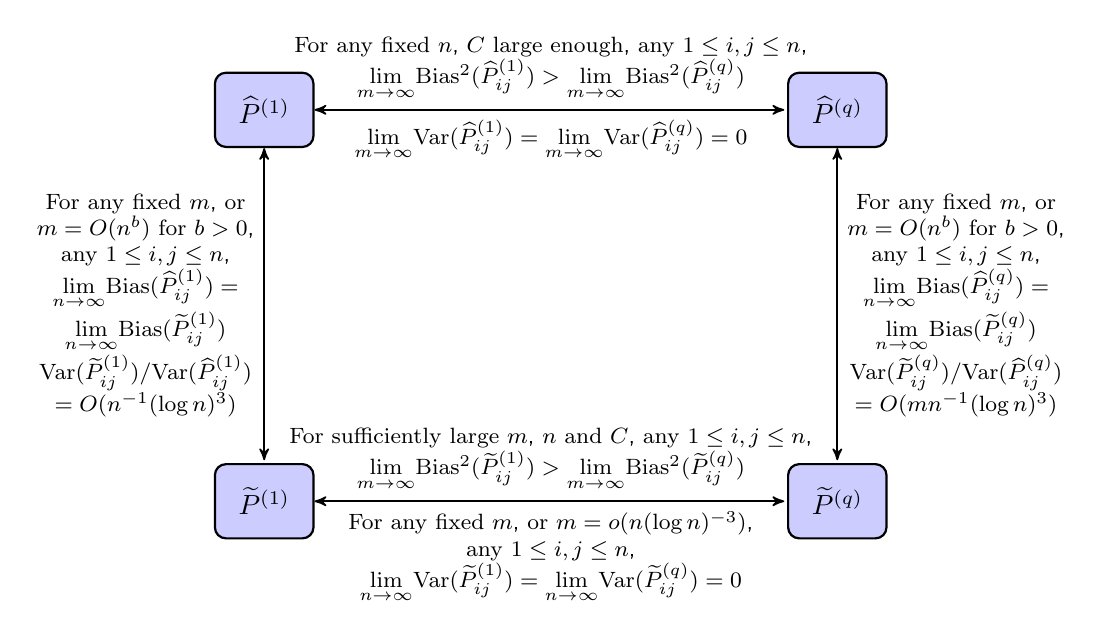
\begin{tikzpicture}[
  font=\sffamily,
  every matrix/.style={ampersand replacement=\&,column sep=2cm,row sep=2cm},
  block/.style={draw,thick,rounded corners,fill=blue!20,inner sep=.3cm},
  process/.style={draw,thick,circle,fill=blue!20},
  sink/.style={source,fill=green!20},
  datastore/.style={draw,very thick,shape=datastore,inner sep=.3cm},
  dots/.style={gray,scale=2},
  to/.style={->,>=stealth',shorten >=1pt,semithick,font=\sffamily\footnotesize},
  tofrom/.style={<->,>=stealth',shorten >=1pt,semithick,font=\sffamily\footnotesize},
  every node/.style={align=center}]

  % Position the nodes using a matrix layout
  \matrix{
    \node[block] (MLE) {$\hat{P}^{(1)}$};
      \& \& \& \node[block] (MLqE) {$\hat{P}^{(q)}$};\\
	\\
    \node[block] (XMLE) {$\widetilde{P}^{(1)}$};
      \& \& \& \node[block] (XMLqE) {$\widetilde{P}^{(q)}$}; \\
  };

  % Draw the arrows between the nodes and label them.
  \draw[tofrom] (MLE) -- node[midway,above] {$\mathrm{For}$ $\mathrm{any}$ $\mathrm{fixed}$ $n$, $C$ $\mathrm{large}$ $\mathrm{enough}$, $\mathrm{any}$ $1 \le i, j \le n$, \\$\underset{m \to \infty}{\lim} \mathrm{Bias}^2(\hat{P}_{ij}^{(1)}) > \underset{m \to \infty}{\lim} \mathrm{Bias}^2(\hat{P}_{ij}^{(q)})$}
      node[midway,below] {$\underset{m \to \infty}{\lim} \mathrm{Var}(\hat{P}_{ij}^{(1)}) = \underset{m \to \infty}{\lim} \mathrm{Var}(\hat{P}_{ij}^{(q)}) = 0$} (MLqE);
  \draw[tofrom] (MLE) -- node[midway,left] {$\mathrm{For}$ $\mathrm{any}$ $\mathrm{fixed}$ $m$, $\mathrm{or}$ \\ $m = O(n^b)$ $\mathrm{for}$ $b>0$, \\$\mathrm{any}$ $1 \le i, j \le n$, \\$\underset{n \to \infty}{\lim} \mathrm{Bias}(\hat{P}_{ij}^{(1)}) =$\\$ \underset{n \to \infty}{\lim} \mathrm{Bias}(\widetilde{P}_{ij}^{(1)})$\\$\mathrm{Var}(\widetilde{P}_{ij}^{(1)})/\mathrm{Var}(\hat{P}_{ij}^{(1)})$\\$ = O(n^{-1} (\log n)^3)$} (XMLE);
  \draw[tofrom] (MLqE) -- node[midway,right] {$\mathrm{For}$ $\mathrm{any}$ $\mathrm{fixed}$ $m$, $\mathrm{or}$ \\ $m = O(n^b)$ $\mathrm{for}$ $b>0$, \\$\mathrm{any}$ $1 \le i, j \le n$, \\$\underset{n \to \infty}{\lim} \mathrm{Bias}(\hat{P}_{ij}^{(q)}) = $\\$\underset{n \to \infty}{\lim} \mathrm{Bias}(\widetilde{P}_{ij}^{(q)})$\\$\mathrm{Var}(\widetilde{P}_{ij}^{(q)})/\mathrm{Var}(\hat{P}_{ij}^{(q)})$\\$= O(m n^{-1} (\log n)^3)$} (XMLqE);
  \draw[tofrom] (XMLE) -- node[midway,above] {$\mathrm{For}$ $\mathrm{sufficiently}$ $\mathrm{ large}$ $m$, $n$ $\mathrm{and}$ $C$, $\mathrm{any}$ $1 \le i, j \le n$, \\$\underset{m \to \infty}{\lim} \mathrm{Bias}^2(\widetilde{P}_{ij}^{(1)}) > \underset{m \to \infty}{\lim} \mathrm{Bias}^2(\widetilde{P}_{ij}^{(q)})$}
      node[midway,below] {$\mathrm{For}$ $\mathrm{any}$ $\mathrm{fixed}$ $m$, $\mathrm{or}$ $m = o(n (\log n)^{-3})$, \\$\mathrm{any}$ $1 \le i, j \le n$, \\$\underset{n \to \infty}{\lim} \mathrm{Var}(\widetilde{P}_{ij}^{(1)}) = \underset{n \to \infty}{\lim} \mathrm{Var}(\widetilde{P}_{ij}^{(q)}) = 0$} (XMLqE);
\end{tikzpicture}
\end{center}
\caption{\label{fig:summary}Relationship among four estimators.}
\end{figure}






\section{Extensions}
\label{section:extension}

Although in Section \ref{section:theory}, we only present the results under exponential distributions, the results can be generalized to a broader class of distribution families, and even a different entry-wise robust estimator other than ML$q$E with the following conditions:
\begin{enumerate}
\item Let $A_{ij} \stackrel{ind}{\sim} (1-\epsilon) f_{P_{ij}} + \epsilon f_{C_{ij}}$, then $E[(A_{ij} - E[\hat{P}_{ij}^{(1)}])^k] \le \mathrm{const} \cdot k!$, where $\hat{P}^{(1)}$ is the entry-wise MLE as defined before;\\
%$E[\hat{P}_{ij}^{(1)}] = (1-\epsilon) E_f(P_{ij}) + \epsilon E_f(C_{ij})$;
This is to ensure the that observations will not deviate from the expectation too far away, such that the concentration inequality can apply.
\item There exists $C_0(P_{ij}, \epsilon) > 0$ such that under the contaminated model with $C > C_0(P_{ij}, \epsilon)$,
\[
	\lim_{m \to \infty} \left| E[\hat{P}_{ij}] - P_{ij} \right| < 
    \lim_{m \to \infty} \left| E[\hat{P}^{(1)}_{ij}] - P_{ij} \right|;
\]\\
This condition is discussed in Section \ref{section:MLEvsMLqE}. It requires the contamination of the model to be large enough (a restriction on the distribution) and $\hat{P}$ to be robust enough with respect to the contamination (a condition on the estimator).
\item $\hat{P}_{ij} \le \mathrm{const} \cdot \hat{P}_{ij}^{(1)}$; (This might be generalized to with high probability later)\\
Since we use the results of $\hat{P}^{(1)}$ to bound $\hat{P}^{(q)}$, the proof can apply directly with this condition for an arbitrary $\hat{P}$.
\item $\mathrm{Var}(\hat{P}_{ij}) = O(m^{-1})$, where $m$ is the number of observations.\\
We will get exactly the same results as in Section \ref{section:theory}. However, even if the variance of the new estimator is not of order $O(m^{-1})$, we will get similar results with a different term related to $m$.
\end{enumerate}


\section{Empirical Results}

\subsection{Simulation Results}

\begin{itemize}
\item In this section, we will illustrate the theoretical results of four estimators in Section \ref{section:theory} via various Monte Carlo simulation experiments.
\end{itemize}

\subsubsection{Simulation Setting}
%\begin{itemize}
%\item Here we consider the 2-block SBM parameterized by
%\begin{equation*}
%B = \begin{bmatrix}
%4.2 & 2 \\
%2 & 7
%\end{bmatrix}
%,\qquad \rho = \begin{bmatrix}
%0.5 & 0.5
%\end{bmatrix}.
%\end{equation*}
%\item The contamination is also a 2-block SBM parameterized by
%\begin{equation*}
%B = \begin{bmatrix}
%20 & 18 \\
%18 & 25
%\end{bmatrix}
%,\qquad \rho = \begin{bmatrix}
%0.5 & 0.5
%\end{bmatrix}.
%\end{equation*}
%\item And we embed the graphs into the dimension $d = \mathrm{rank}(B) = 2$.
%\end{itemize}

\begin{itemize}
\item Here we consider the 3-block SBM with respect to the exponential distributions parameterized by
\begin{equation*}
B = \begin{bmatrix}
4.2 & 2 \\
2 & 7
\end{bmatrix}
,\qquad \rho = \begin{bmatrix}
0.5 & 0.5
\end{bmatrix}.
\end{equation*}
\item The contamination is also a 3-block SBM with respect to the exponential distributions parameterized by
\begin{equation*}
B^{\prime} = \begin{bmatrix}
20 & 18 \\
18 & 25
\end{bmatrix}
,\qquad \rho = \begin{bmatrix}
0.5 & 0.5
\end{bmatrix}.
\end{equation*}
\item And we embed the graphs into the dimension $d = \mathrm{rank}(B) = 2$.
\end{itemize}


\subsubsection{Simulation Results}
\begin{itemize}
\item Figure \ref{fig:eps} plots the mean squared error in average by varying contamination ratio $\epsilon$ with fixed $n = 100$ and $m = 10$ based on 1000 Monte Carlo replicates. And we use $q=0.8$ when applying ML$q$E.
Different colors represent the simulated MSE associated with four different estimators.
\textbf{1. MLE $\hat{P}^{(1)}$ vs ML$q$E $\hat{P}^{(q)}$:}
MLE outperforms a little bit when there is no contamination (i.e. $\epsilon = 0$), but it degrades dramatically when contamination increases;
\textbf{2. MLE $\hat{P}^{(1)}$ vs ASE o MLE $\widetilde{P}^{(1)}$: }
ASE procedure takes the low rank structure into account and $\widetilde{P}^{(1)}$ wins the bias-variance tradeoff;
\textbf{3. ML$q$E $\hat{P}^{(q)}$ vs ASE o ML$q$E $\widetilde{P}^{(q)}$: }
ML$q$E preserves the low rank structure of the original graph more or less, so ASE procedure still helps and $\widetilde{P}^{(q)}$ wins the bias-variance tradeoff;
\textbf{4. ASE o ML$q$E $\widetilde{P}^{(q)}$ vs ASE o MLE $\widetilde{P}^{(1)}$: }
When contamination is large enough, $\widetilde{P}^{(q)}$ based on ML$q$E is better, since it inherits the robustness from ML$q$E.
\item Figure \ref{fig:q} show the mean squared error in average by varying the parameter $q$ in ML$q$E with fixed $n = 100$, $m = 10$ and $\epsilon = 0.2$ based on 1000 Monte Carlo replicates. Different colors represent the simulated MSE associated with four different estimators.
1. ASE procedure takes advantage of the graph structure and improves the performance of the corresponding estimators;
2. ML$q$E shows the robustness property compare to the MLE. And as $q$ goes to 1, ML$q$E goes to the MLE as expected.
\item By comparing the performance of the four estimators based on different setting, we demonstrate the theoretical results in Section \ref{section:theory}.
\end{itemize}

\begin{figure}[!htb]
\centering
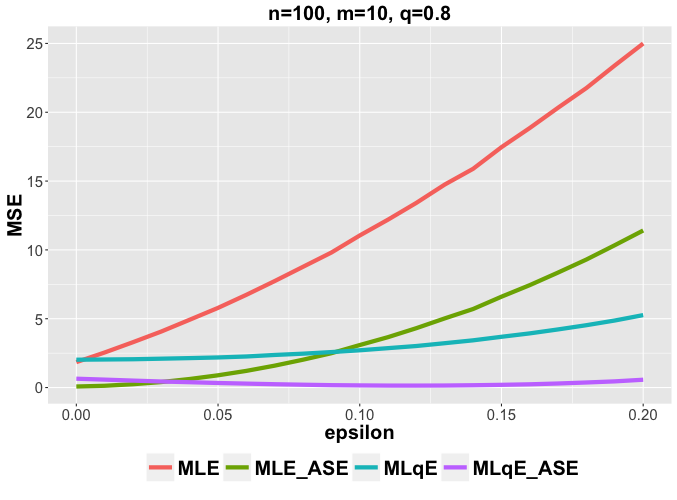
\includegraphics[width=1\textwidth]{eps.png}
\caption{Mean squared error in average by varying contamination ratio $\epsilon$ with fixed $n = 100$ and $m = 10$ based on 1000 Monte Carlo replicates. And we use $q=0.8$ when applying ML$q$E.
Different colors represent the simulated MSE associated with four different estimators.
\textbf{1. MLE $\hat{P}^{(1)}$ vs ML$q$E $\hat{P}^{(q)}$:}
MLE outperforms a little bit when there is no contamination (i.e. $\epsilon = 0$), but it degrades dramatically when contamination increases;
\textbf{2. MLE $\hat{P}^{(1)}$ vs ASE o MLE $\widetilde{P}^{(1)}$: }
ASE procedure takes the low rank structure into account and $\widetilde{P}^{(1)}$ wins the bias-variance tradeoff;
\textbf{3. ML$q$E $\hat{P}^{(q)}$ vs ASE o ML$q$E $\widetilde{P}^{(q)}$: }
ML$q$E preserves the low rank structure of the original graph more or less, so ASE procedure still helps and $\widetilde{P}^{(q)}$ wins the bias-variance tradeoff;
\textbf{4. ASE o ML$q$E $\widetilde{P}^{(q)}$ vs ASE o MLE $\widetilde{P}^{(1)}$: }
When contamination is large enough, $\widetilde{P}^{(q)}$ based on ML$q$E is better, since it inherits the robustness from ML$q$E.}
\label{fig:eps}
\end{figure}

\begin{figure}[!htb]
\centering
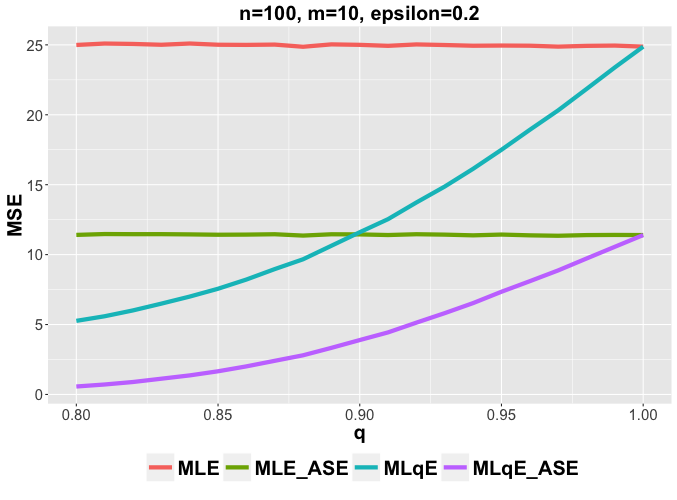
\includegraphics[width=1\textwidth]{q.png}
\caption{Mean squared error in average by varying the parameter $q$ in ML$q$E with fixed $n = 100$, $m = 10$ and $\epsilon = 0.2$ based on 1000 Monte Carlo replicates. Different colors represent the simulated MSE associated with four different estimators.
1. ASE procedure takes advantage of the graph structure and improves the performance of the corresponding estimators;
2. ML$q$E shows the robustness property compare to the MLE. And as $q$ goes to 1, ML$q$E goes to the MLE as expected.}
\label{fig:q}
\end{figure}

  
%\begin{figure}
%\centering
%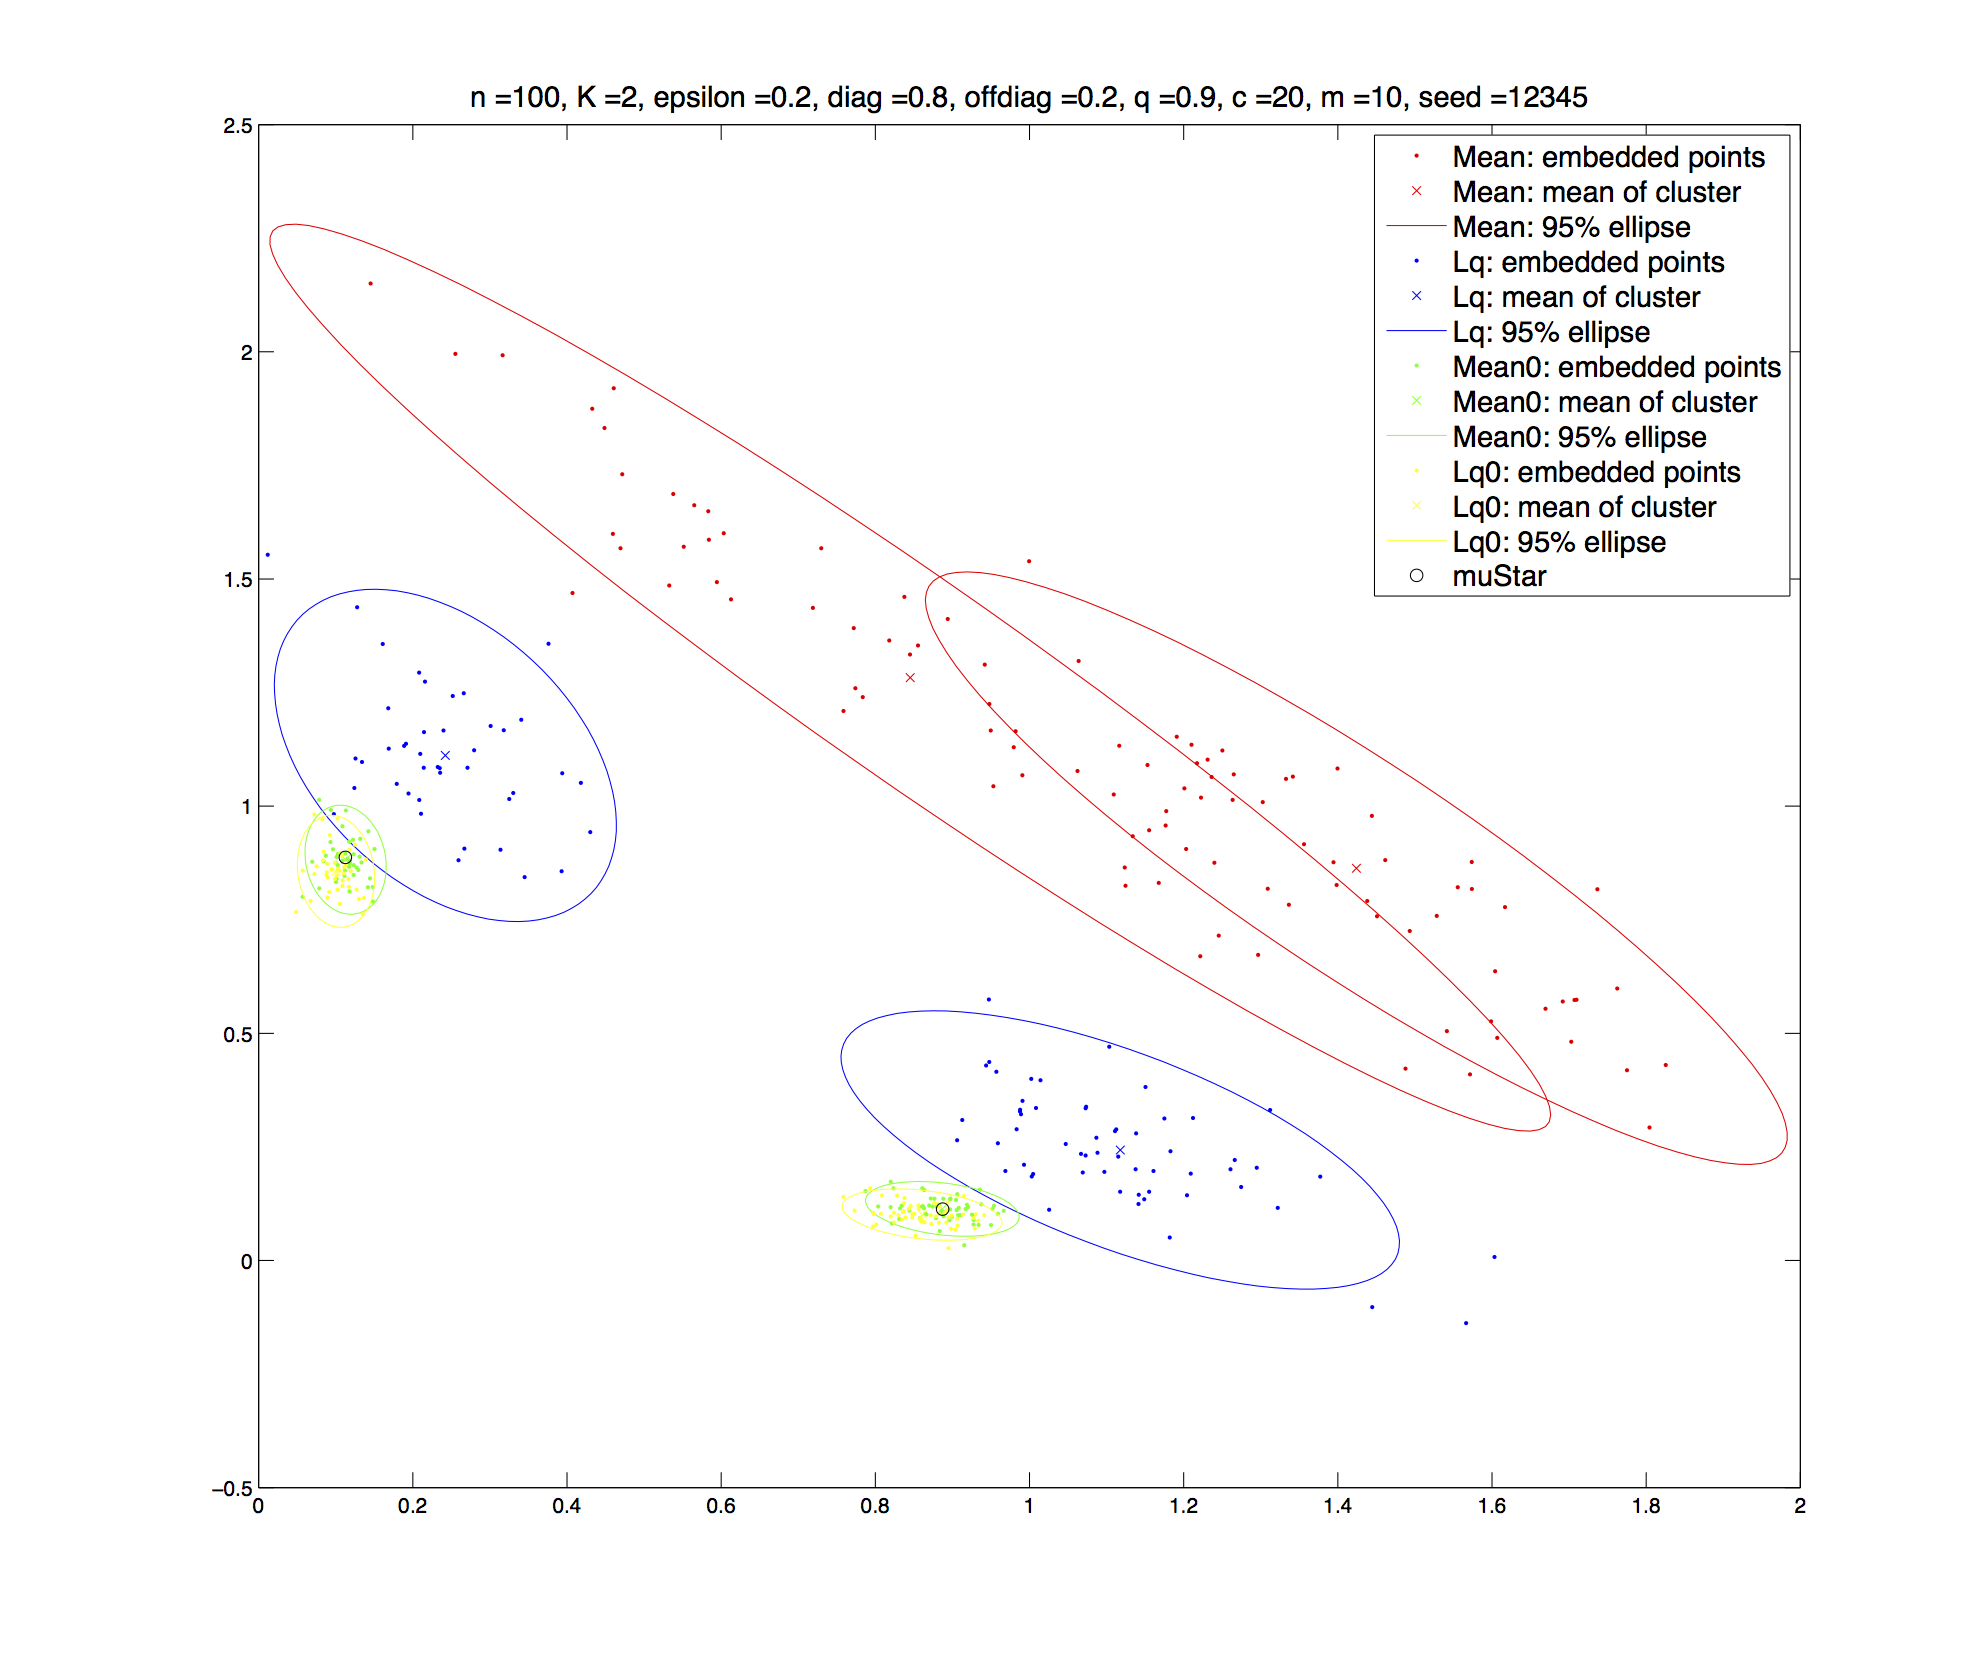
\includegraphics[width=0.8\textwidth]{Cluster.png}
%\end{figure}



\subsection{CoRR Graphs}
\label{section:real_data}
\begin{itemize}
\item In practice, the graphs may not perfectly follow an RDPG, or even not IEM. But we are still interested in the performance of the four estimators. In this work, we examine the structural connectomic data. The graphs are based on diffusion tensor MR
images. It contains 114 different brain scans, each of which was processed to yield an undirected, weighted graph with no
self-loops, using the m2g pipeline described in \citet{kiar2016ndmg}. The vertices of the graphs represent different regions in the brain defined according to an atlas. We used the desikan atlas with 70 vertices. The weight of an edge between two vertices represents the number of white-matter tract connecting the corresponding two regions of the brain.
\item We first check if the dataset has the low-rank property. In the left panel of Fig.~\ref{fig:screehist}, we plot the eigenvalues of the mean graph of all 114 graphs (with diagonal augmentation) in decreasing algebraic order for the Desikan atlases based on the m2g pipeline. The eigenvalues first decrease dramatically and then stay around 0 for a large range of dimensions. In addition, we also plot the histograms in the right panel of Fig.~\ref{fig:screehist}. From the figures we can see many eigenvalues are around zero, with a few large eigenvalues. So the information is mostly contained in the first few dimensions. Such quasi low-rank property could be used.
\item To compare the four estimators, we need to know the true parameter matrix $P$. However, $P$ is definitely not obtainable in practice since the 114 graphs are also a sample from the population. In this work, we are going to use two different approaches to approximate the the probability matrix $P$.
\item First, we assume that the true probability matrix $P$ has the low-rank property. In this case, the low-rank approximation of the mean graph of all 114 graphs is a good estimate of the probability matrix $P$.
We admit that this setting is preferable by the low-rank estimators. However, it is illustrative to see how the estimators perform in this case.
\item In the above setting, we run 100 simulations on the dataset for each sample size $m = 2$, $m = 5$, and $m = 10$.
Specifically, for each Monte Carlo replicate, we sample $m$ graphs out of the 114 from the m2g dataset and computing the four estimates based on the $m$ sampled graphs. We then compared these estimates to the low-rank approximation of the mean of all 114 graphs from the m2g dataset.
For those two low-rank estimators, we apply ASE for all possible dimensions, i.e. $d$ ranges from 1 to $n$. The result is shown in Figure \ref{fig:CCI_LR}.
\item Since the approximated $P$ contains outliers, we don't expect ML$q$E helps much as shown in the figure. However, since the estimated $P$ has the low-rank property, ASE procedure helps improving the performance. The dimensions chosen by the 3d elbow of Zhu and Ghodsi are denoted in triangle and square. We can see it does a good job. More importantly, a wide range of dimensions could lead to an improvement.

\begin{figure}[!htbp]
\centering
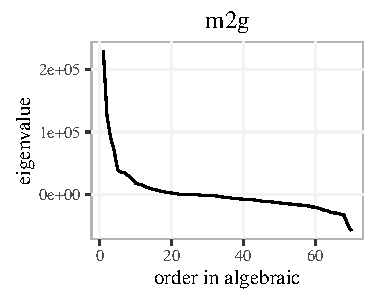
\includegraphics[height=.2\textheight]{screeplot_m2g.pdf}
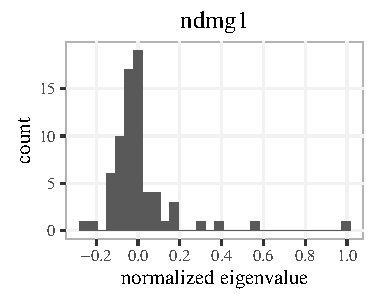
\includegraphics[height=.2\textheight]{hist_m2g.pdf}
\caption{{\bf Screeplot and the histogram of the eigenvalues of the  mean of 114 graphs based on m2g pipeline.}
The screeplot in the left panel shows the eigenvalues of the mean graph of all 114 graphs with diagonal augmentation in decreasing algebraic order for the Desikan atlas. The right panel shows the histogram of the eigenvalues of the mean graph of all 114 graphs with diagonal augmentation. Many eigenvalues are around zero, which lead to a quasi low-rank structure.
}
\label{fig:screehist}
\end{figure}

\begin{figure}
\centering
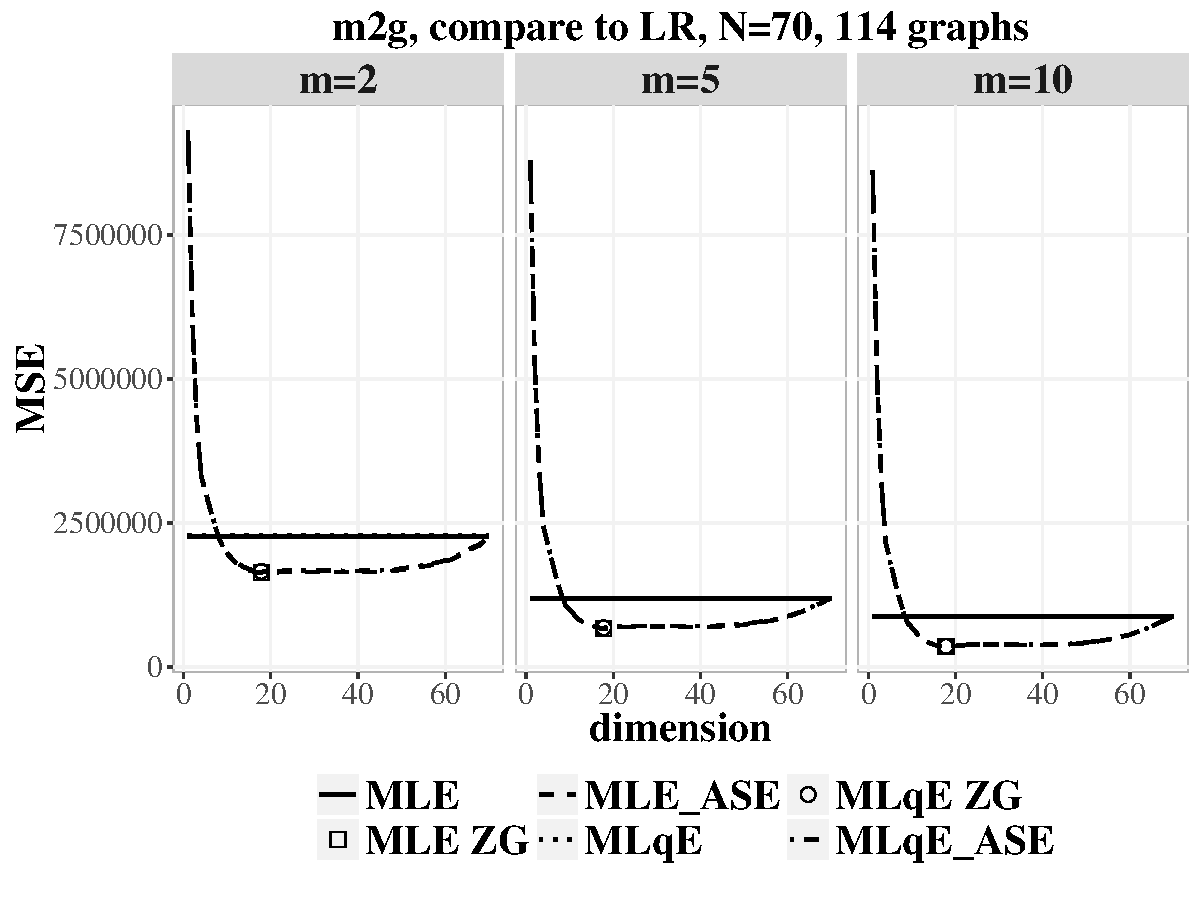
\includegraphics[width=0.8\textwidth]{CCI_CompareLR.pdf}
\caption{Comparison of mean squared error in average among four estimators while embedding the graphs into different dimensions with different size $m$ of the subsamples by using the low-rank approximation of the mean of the rest $114 - m$ graphs as the approximation of $P$. Four estimators are represented by different line styles as explained in the legend. Since the approximated $P$ contains outliers, we don't expect ML$q$E helps much as shown in the figure. However, since the estimated $P$ has the low-rank property, ASE procedure helps improving the performance. The dimensions chosen by the 3rd elbow of Zhu and Ghodsi are denoted in triangle and square. We can see it does a good job. More importantly, a wide range of dimensions could lead to an improvement.}
\label{fig:CCI_LR}
\end{figure}

\item Also, we consider a setting which is favorable to the MLE, i.e. assuming that the probability matrix $P$ has a high-rank property. Since we know ndmg2 is a better pipeline compared to m2g, the mean graph derived from ndmg2 should be a relative accurate estimate of the actual population mean graph. Since the mean of 114 graphs has full rank, it breaks the low-rank assumptions and are favorable to the MLE.
In order to evaluate the performance of the four estimators, we build estimates based on the samples with size $m$ from the m2g dataset, while using the sample mean of all 114 graphs from the ndmg2 dataset as an estimate of the probability matrix $P$.
\item We run 100 simulations on the dataset for each sample size $m = 2$, $m = 5$, and $m = 10$.
Specifically, for each Monte Carlo replicate, we sample $m$ graphs out of the 114 from the m2g dataset and computing the four estimates based on the $m$ sampled graphs. We then compared these estimates to the mean of all 114 graphs in the ndmg2 dataset.
For those two low-rank estimators, we apply ASE for all possible dimensions, i.e. $d$ ranges from 1 to $n$. The result is shown in Figure \ref{fig:CCI}.
\item Since it is real data, ML$q$E outperforms ML$E$ because of the robustness property. Moreover, as suggested in the previous theorems, such property is kept after the ASE procedure.
\item When $d$ is small, ASE procedure underestimates the dimension and fails to get important information, which leads to poor performance. In practice, we use algorithms like Zhu and Ghodsi's method to select the dimension $d$. We can see Zhu and Ghodsi's algorithm does a pretty good job for selecting the dimension to embed.
\item For all three sample sizes ($m = 2$, $m = 5$, $m = 10$), MLE and ML$q$E have large variances which lead to large MSE. Meanwhile, the ASE procedure reduces the variance by taking advantages of the graph structure.
\end{itemize}






\begin{figure}
\centering
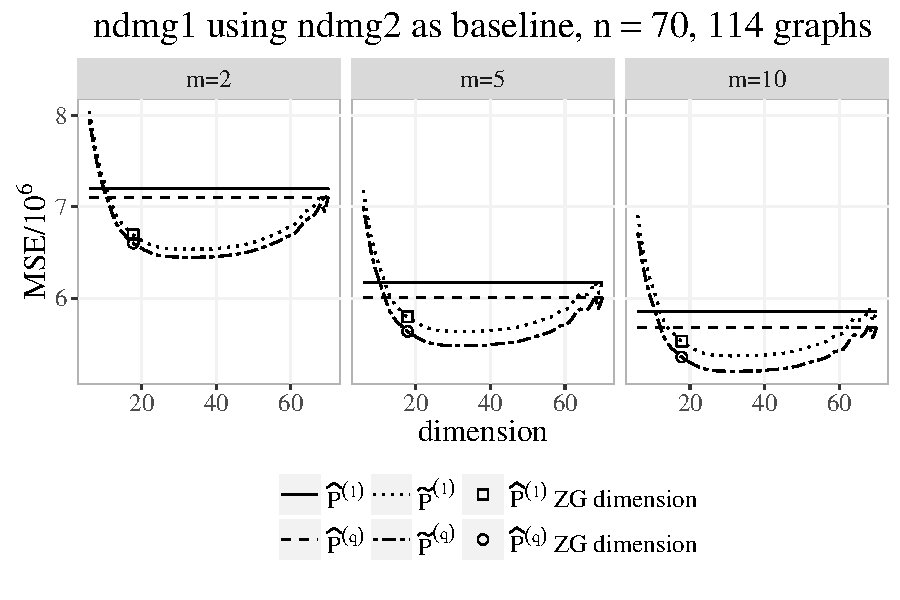
\includegraphics[width=\textwidth]{CCI.pdf}
\caption{{\bf Comparison of MSE of the four estimators for the desikan atlases at three sample sizes based on m2g and ndmg2 pipelines.}  
{\bf 1. MLE (horizontal solid line) vs MLqE (horizontal dotted line):} 
ML$q$E outperforms MLE since robust estimators are always preferred in practice;
{\bf 2. MLE (horizontal solid line) vs MLE\_ASE (dashed line):} MLE\_ASE wins the bias-variance tradeoff when embedded into a proper dimension; 
{\bf 3. MLqE (horizontal dotted line) vs ML$q$E\_ASE (dashed dotted line):}
ML$q$E\_ASE wins the bias-variance tradeoff when embedded into a proper dimension; 
{\bf 4.  ML$q$E\_ASE (dashed dotted line) vs MLE\_ASE (dashed
line):}
MLqE\_ASE is better, since it inherits the robustness from 
ML$q$E. And the square and circle represent the dimensions selected by the Zhu and Ghodsi method. We can see it does a pretty good job. And more importantly, a wide range of dimensions could lead to an improvement.
}
\label{fig:CCI}
\end{figure}






\section{Discussion}


\section{Appendix}

All proofs here.



\bibliography{Bib}{}
%\bibliographystyle{plain}
\bibliographystyle{plainnat}






%\newpage
%
%\section{Backup}
%
%
%\section{Discussion}
%
%\subsection{Summary}
%\begin{itemize}
%\item In this paper, we propose a better way to estimate the mean of a collection of graphs by taking advantage of the low rank structure of the graphs.
%\end{itemize}
%
%\subsection{Future Work}
%\begin{itemize}
%\item Generally the observations we have are always contaminated in practice. In this case, improved robust estimator based on the low rank structure of the graphs is preferred.
%\item Estimating the rank of the graph structure accurately will certainly help improve the results.
%\item In this paper, we are using Scheinerman's method with 1 iteration for diagonal augmentation.
%\end{itemize}
%
%
%
%
%
%
%\section{Methods}
%
%\subsection{Choosing Dimension}
%\label{section:dim_select}
%\begin{itemize}
%\item Often in dimensionality reduction techniques, the choice for dimension, d, relies on visually analyzing a plot of the ordered eigenvalues, looking for a ``gap'' or ``elbow'' in the scree-plot.
%\item USVT is a simple estimation procedure that works for any matrix that has ``a little bit of structure''.
%\end{itemize}
%
%\subsection{Graph Diagonal Augmentation}
%\begin{itemize}
%\item The graphs examined in this work are hollow, in that there are no self-loops and thus the diagonal entries of the adjacency matrix are 0. This leads to a bias in the calculation of the eigenvectors.
%\item We minimize this bias by using an iterative method developed by Scheinerman and Tucker.
%\end{itemize}
%
%\subsection{Source Code}
%
%\subsection{Dataset Description}
%\begin{itemize}
%\item The original dataset is from the Emotion and Creativity One Year Retest Dataset provided by Qiu, Zhang and Wei from Southwest University. It is comprised of 235 subjects, all of whom were college students. Each subject underwent two sessions of anatomical, resting state DTI scans, spaced one year apart. Due to the incomplete data, the true number of scans is 454.
%\item When deriving MR connectomes, the NeuroData team parcellate the brain into groups of nodes as defined by anatomical atlases. The atlases are defined either physiologically or structurally by neuroanatomists (Desikan and JHU), or are generated using a segmentation algorithm looking for certain features or groupings (CPAC200).
%\item The graphs we are using are processed by NeuroData team from DTI data of the original dataset generated with different atlases (desikan, JHU and CPAC200), each containing different region/node definitions.
%\item The graphs are undirected, unweighted and with no self-loops. An edge exists between two regions when there is at least one white-matter tract connecting the corresponding two parts of the brain.
%\end{itemize}
%
%\subsection{Outline for the Proof of the Theorems}



\end{document}